\documentclass[11pt]{article}

\input{preamble} % If needed, you can load additional packages or
% define your own macros in the preamble.tex file

\title{VesSkel: Vessel Skeletonization and Graph-Based Phenotype Analysis in
Retinal Fundus Images}
\author{Simon Wittmann}

\affil{
  % [Master's / Bachelor's] thesis in [your study degree]\\ % For theses
  % Direct supervisor: [your direct thesis supervisor]\\ % For theses,
  % delete if directly supervised by David
  % Supervising professor: Prof. Dr. David B. Blumenthal\\ % For theses
  Project report\\ % For project reports in the module Project
  Biomedical Network Science\\
  %Student paper\\ % For student papers in the module Network Medicine
  Module title: Project Biomedical Network Science\\
  Semester: SS 2026\\
  Matriculation number: 23760671\\
  Biomedical Network Science Lab, Department Artificial Intelligence in
Biomedical Engineering, Friedrich-Alexander-Universität Erlangen-Nürnberg}

\date{Submission date: [date]}

\begin{document}

\maketitle

\begin{abstract}
  Write your abstract here. An abstract is a brief one-paragraph
  summary that motivates your work, and provides a high-level
  description of why it is relevant. Excellent guidelines can be
  found here:
  \url{https://www.nature.com/documents/nature-summary-paragraph.pdf}.
  Your abstract should fit on the first page of this document.
\end{abstract}

\clearpage

\tableofcontents

\clearpage

\section{Introduction}\label{sec:introduction}

The retina is the only organ where the microvasculature can be imaged
non-invasively using fundus photography~\cite{HRF}. Quantitative
analysis of retinal vessel morphology provides clinically relevant
biomarkers for systemic and ocular diseases such as diabetic
retinopathy and glaucoma~\cite{improved_turtosity}. To extract
these biomarkers from binary vessel segmentations, a common approach
is to skeletonize the vessel mask and then derive graph-based
features from the resulting one-pixel-wide centerline representation.

Several software tools have been developed for this task, including
REAVER~\cite{REAVER}, VesselVio~\cite{VesselVio},
VesselExpress~\cite{VesselExpress}, TWOMBLI~\cite{TWOMBLI},
VesSAP~\cite{VesSAP}, and Skan~\cite{Skan<3}. These tools differ
substantially as can be seen in Table~\ref{tab:tools-general}.

\begin{table}[htb]
  \centering
  \caption{Comparison of Different Vessel Processing
  Tools}\label{tab:tools-general}
  \small
  \begin{tabularx}{\textwidth}{lXXXXXX}
    \toprule
    Feature & REAVER & VesselVio & VesselExpress & TWOMBLI & VesSAP & Skan\\
    \midrule
    2D/3D & 2D & both & 3D & 2D & 3D & both\\
    \midrule
    GUI/Interface & interactive Matlab GUI & PyQt5 standalone app +
    cli & Web App (Docker) and Napari Plugin & FIJI/ImageJ Plugin
    with guided param setup & CLI only & Napari Plugin and Python Package\\
    \midrule
    Input Type & Raw 2D fluorescent images & Pre-binarized datasets &
    Raw 3D Volumes & Raw 2D Images & Raw 3D Volume & Pre-skeletonized binary\\
    \midrule
    License & BSD 3.0 & GPLv. 3 & GPLv. 3 & ? & MIT & BSD 3-clause\\
    \midrule
    Segmentation & Auto (background sub + adaptive threshold +
    morphological) & None & Auto (dual Frangi filter + statistical
    threshold) & Auto (Steger ridge detection) & Auto (5-layer 3D
    CNN, transfer learning) & None (skeleton analysis only)\\
    \midrule
    Skeletonization & Matlab bwmorph & Lee94 (custom numba impl) &
    skimage lee94 & None & skimage lee94 & None\\
    \bottomrule
  \end{tabularx}
\end{table}

Despite their individual strengths, no existing tool
simultaneously offers (i)~a permissive (MIT) license, (ii)~support
for both 2D and 3D binary masks, (iii)~an interactive graphical
interface alongside a batch-processing CLI, and (iv)~a comprehensive
feature set that includes fractal dimension, per-segment radius
statistics, and automatic cleanup of skeletonization artifacts. This
fragmentation forces researchers to maintain heterogeneous,
multi-tool pipelines that hinder reproducibility and increase the
barrier to entry for quantitative vessel analysis.

We present VesSkel, an MIT-licensed Python package for vessel
skeletonization and graph-based phenotype analysis. VesSkel
implements the Lee94 thinning algorithm~\cite{lee94} with Numba-based
parallelization, supporting both 2D and 3D binary masks. The output
is verified to be pixel-identical to scikit-image's Lee94
implementation. In 2D benchmarks on the 45-image HRF dataset, VesSkel
achieves a mean thinning time of 0.084~s per image, outperforming
scikit-image's Lee (0.438~s, 5.2$\times$ slower) and VesselVio's Lee
(0.796~s, 9.5$\times$ slower). In 3D, VesSkel (0.730~s) is
competitive with scikit-image (1.024~s) and VesselVio (0.804~s).
Beyond thinning, VesSkel provides an end-to-end pipeline: optional
preprocessing (morphological closing and hole-filling), Lee94
skeletonization, a novel junction-cleanup step that removes
thinning-induced triangle artifacts on the skeleton graph, graph
construction using Skan~\cite{Skan<3}, and extraction of per-image,
per-branch, and per-node features.

VesSkel computes 29 summary features covering vessel topology (node
count, edge count, bifurcations, connected components), morphology
(segment lengths, tortuosity, radii, fractal dimension, hyphal growth
unit), and density (vessel area fraction). Per-branch and per-node
features provide additional granularity for localized analyses. The
entire pipeline is accessible through two complementary interfaces: a
napari plugin for interactive parameter tuning and visual feedback,
and a command-line interface for reproducible batch processing. All
extraction and output settings are serializable to a JSON configuration
file, enabling full experiment reproducibility.

We demonstrate VesSkel on the High-Resolution Fundus (HRF)
dataset~\cite{HRF}, which comprises 45 fundus images with manual
vessel segmentations from three clinical groups: 15 healthy subjects,
15 patients with diabetic retinopathy, and 15 patients with glaucoma.
From each image, we extracted the full set of vessel phenotype
features and evaluated their discriminative power using analysis of
variance (ANOVA) and multi-class classification. Support vector
machine classification with stratified 5-fold cross-validation
achieves 91.1\% accuracy (linear kernel, $C=0.1$, top-10 features
selected by ANOVA F-statistic), outperforming logistic regression
(88.9\%) and random forest (82.2\%). These results confirm that the
features captured by VesSkel encode biologically relevant differences
in retinal vasculature.

In summary, our main contributions are: (1)~a Numba-parallelized
Lee94 thinning implementation for 2D and 3D data, validated for
correctness against scikit-image and benchmarked against existing
implementations; (2)~an integrated feature extraction pipeline with a
novel junction artifact cleanup mechanism; (3)~a dual-interface
design (napari plugin + CLI) with JSON-configurable reproducibility;
and (4)~a demonstration of phenotype differentiation and
classification on the HRF dataset. The remainder of this paper is
organized as follows. Section~\ref{sec:results} presents the pipeline
overview, skeletonization performance, feature summary, and phenotype
analysis results. Section~\ref{sec:discussion} discusses limitations
and future directions. Section~\ref{sec:methods} details the Lee94
algorithm, our implementation and test strategy, the cleanup
procedure, graph construction, and experimental setup.

\section{Results}\label{sec:results}

% \subsection{Structure of the Results section}\label{sec:results:overview}
%
% The first subsection of the \nameref{sec:results} is often used to
% provide a high-level overview of the entire work. This is typically
% supported by a visual overview in \Cref{fig:overview-placeholder}.
% The overview should enable readers to understand the material
% presented in the subsequent subsections of the \nameref{sec:results}
% section. The methodological details are then explained in a dedicated
% \nameref{sec:methods} section.
%
% \begin{figure}[htb]
%   \centering
%   \includegraphics[width=0.5\linewidth]{example-image-a}
%   \caption{Placeholder for a figure that visualizes the entire study.}
%   \label{fig:overview-placeholder}
% \end{figure}
%
% The remainder of the \nameref{sec:results} is typically structured
% into topical subsections. As a rule of thumb, each subsection should
% present one key finding, supported by one data figure. Of course, you
% can divert from this rule of thumb if it does not fit for your work.
%
% \subsection{Figures}\label{sec:results:figures}
%
% An example of a well-made data figure is shown in
% \Cref{fig:data-figure}. Please ensure that font sizes are large
% enough, that all colors are resolved with legends, and that all $x$-
% and $y$-axes are labeled. If possible, use vector graphics to avoid
% problems due to low resolutions. Add labels to the individual panels
% shown in your figure, which you can then use in your textual
% descriptions. E.\,g.: ``For the multi-class datasets LT1 and LT2
% (\Cref{fig:data-figure}B, C), differences in performance between the
% MLP and SOM classifiers are much more pronounced than for the binary
% datasets LT1b and LT2b (\Cref{fig:data-figure}E, F)''. Place the
% figures in the vicinity of the corresponding text by choosing the
% appropriate placement option. For instance, the placement option
% \verb|htb| used for \Cref{fig:data-figure} tells \LaTeX{} that the
% figure should be placed ``here'' (\verb|h|, preferred choice), at the
% top (\verb|t|, second choice), or at the bottom (\verb|b|, third choice).
%
% \begin{figure}[htb]
%   \centering
%   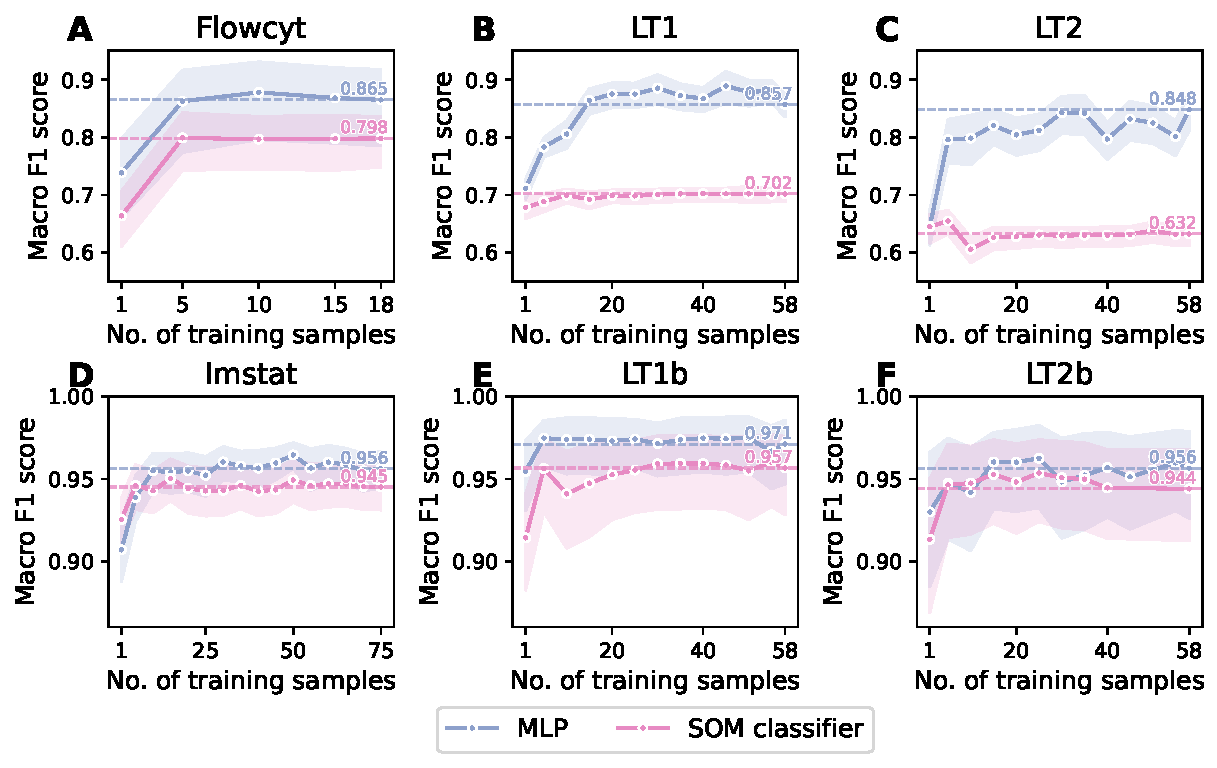
\includegraphics[width=\linewidth]{figures/example_figure.pdf}
%   \caption{Example of a data figure. Figure captions are placed below
%   the figures.}
%   \label{fig:data-figure}
% \end{figure}
%
% \subsection{References}\label{sec:results:references}
%
% References should be included using \verb|\textcite{ID}| and
% \verb|\cite{ID}| as in the following examples, (\verb|ID| is the
% handle of a publication defined in the file ``references.bib''). This
% produces references as in the following examples:
% \textcite{mcinnes2020umap} presented UMAP, a widely used
% dimensionality reduction method. scGPT \cite{Cui2024-km} is one of
% the earliest foundation models for single-cell RNA sequencing data.
%
% \subsection{Tables}\label{sec:results:tables}
%
% \begin{table}[htb]
%   \centering
%   \caption{Caption of \Cref{tab:supp-table}. Table captions are
%   placed above the tables.}
%   \label{tab:supp-table}
%   \begin{tabularx}{\linewidth}{lllX}
%     \toprule
%     Dataset & \# Samples & \# Features & Target variables \\
%     \midrule
%     D1 & 9473 & 187 & Five-year survival rate (binary) and overall
%     survival times (numeric)\\
%     D2 & 94734 & 1837 & Five-year survival rate (binary) and overall
%     survival times (numeric)\\
%     \bottomrule
%   \end{tabularx}
% \end{table}
%
% Nicely formatting tables with \LaTeX{} is a bit tricky, but it is
% possible. \Cref{tab:supp-table} shows an example that uses an
% \verb|X| column from the \verb|tabularx| environment for cells with
% automatic line break that adapt to the available horizontal space, as
% well as the \verb|\toprule|, \verb|\midrule|, and \verb|\bottomrule|
% commands from the \verb|booktabs| package. As for figures, use
% appropriate placement options to ensure that tables appear close to
% the corresponding text.

\subsection{Overview of the VesSkel Pipeline}\label{sec:results:overview}

\begin{figure}[htb]
  \centering
  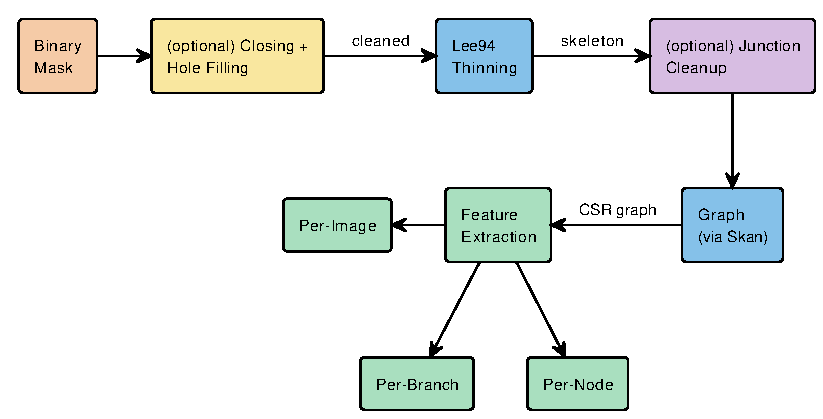
\includegraphics[width=0.9\linewidth]{figures/pipeline_overview.pdf}
  \caption{VesSkel processing pipeline}
  \label{fig:pipeline}
\end{figure}

VesSkel provides an end-to-end pipeline from binary vessel masks to
quantitative phenotype features, as illustrated in
Figure~\ref{fig:pipeline}. The pipeline accepts pre-binarized vessel
segmentations and optionally applies preprocessing (morphological
closing and hole filling) to remove segmentation artifacts. The
cleaned mask is then skeletonized using the Lee94 thinning
algorithm~\cite{lee94}. An optional junction-cleanup step detects and
removes thinning-induced triangle artifacts from the skeleton graph.
The cleaned skeleton is converted to a graph representation using
Skan~\cite{Skan<3}, from which features are extracted at three
granularity levels: per-image summary statistics, per-branch
measurements, and per-node topological properties.

The pipeline is accessible through two complementary interfaces: a
napari plugin for interactive parameter tuning with real-time visual
feedback, and a command-line interface for reproducible batch
processing. All extraction parameters are serializable to a
configuration file, enabling full experiment reproducibility.

\subsection{Preprocessing and Artifact Removal}\label{sec:results:cleanup}

Binary vessel segmentations from automatic or manual annotation
frequently contain small holes and gaps, particularly in regions where
vessels are faint or at vessel crossings. During skeletonization, these
holes cause the thinning algorithm to trace circular paths around their
boundaries, producing spurious loops in the resulting skeleton graph.
To prevent such artifacts, VesSkel applies morphological closing
followed by hole filling as an optional preprocessing step before
thinning. The hole filling operation fills all enclosed background
regions in the mask. Holes exceeding a configurable size threshold are
reverted to preserve legitimate anatomical voids.

\begin{figure}[htb]
  \centering
  \begin{subfigure}[b]{0.3\linewidth}
    
\includegraphics[width=\linewidth]{figures/hole_filling_input_mask.png}
    \caption{Input mask with hole}
    \label{fig:hole_filling:a}
  \end{subfigure}
  \hfill
  \begin{subfigure}[b]{0.3\linewidth}
    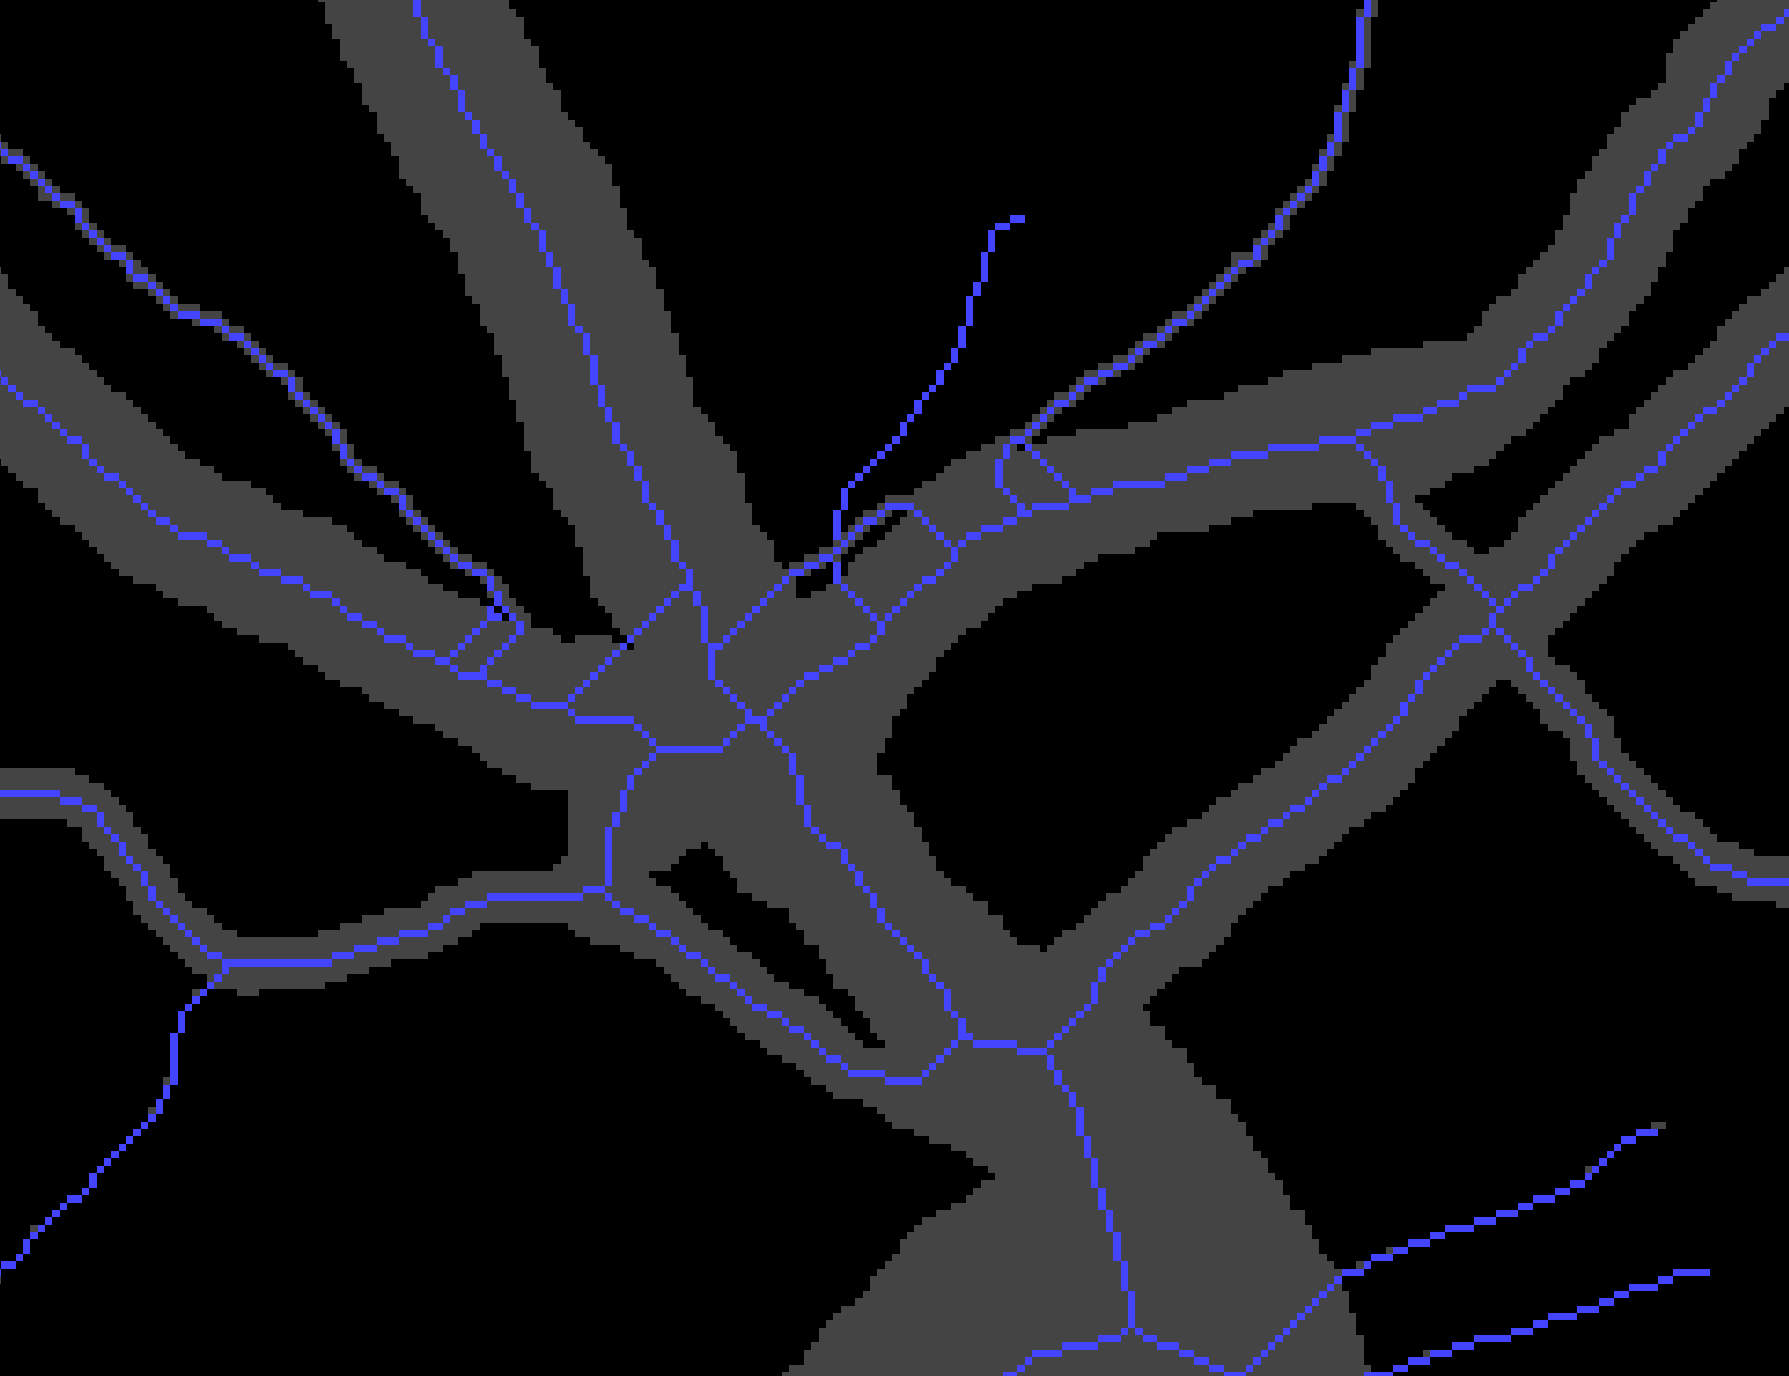
\includegraphics[width=\linewidth]{figures/no_hole_filling_skeleton.png}
    \caption{Without hole filling}
    \label{fig:hole_filling:b}
  \end{subfigure}
  \hfill
  \begin{subfigure}[b]{0.3\linewidth}
    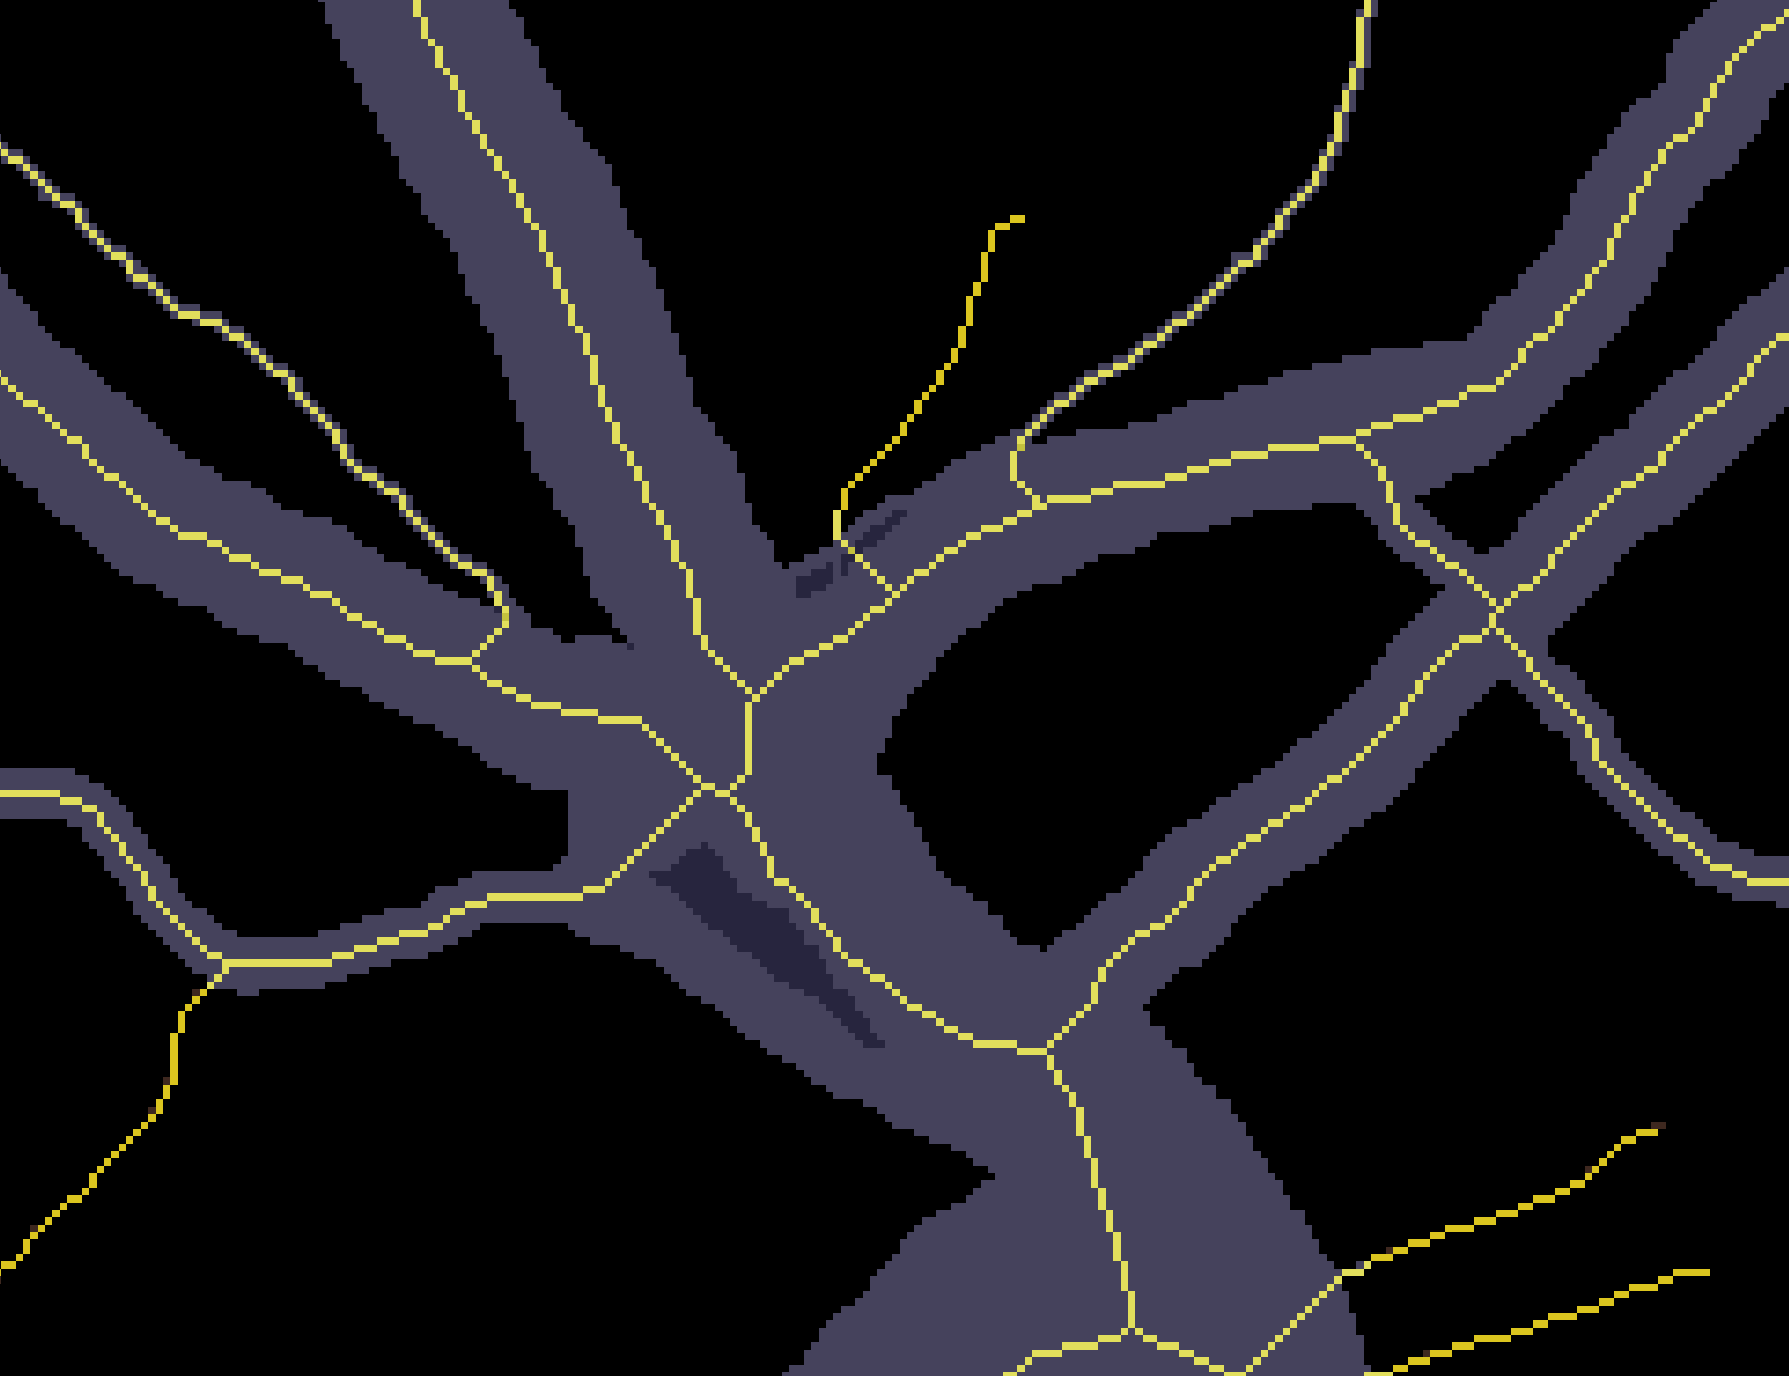
\includegraphics[width=\linewidth]{figures/hole_filling_skeleton.png}
    \caption{With hole filling}
    \label{fig:hole_filling:c}
  \end{subfigure}
  \caption[Effect of hole filling on skeletonization quality]{Effect of
    hole filling on skeletonization quality. (a) Input segmentation mask
    with holes inside a vessel. (b) Without hole filling, the thinning
    algorithm traces the hole boundaries, creating circular skeleton
    artifacts. (c) After hole filling, the skeleton follows the correct
  vessel centerline.}
  \label{fig:hole_filling}
\end{figure}

Figure~\ref{fig:hole_filling} demonstrates the effect on a
representative region of an HRF fundus image. The input segmentation
mask (Figure~\ref{fig:hole_filling}a) contains holes in the vessel
segment, creating circular skeleton artifacts when thinned
directly (Figure~\ref{fig:hole_filling}b). With hole filling, the
skeleton follows the correct vessel centerline without spurious loops
(Figure~\ref{fig:hole_filling}c).

Despite preprocessing, a small number of artifacts may persist after
thinning. The most common are triangle/diamond artifacts at junction
points, which arise from the discrete marching behavior of the
thinning algorithm at bifurcation sites. VesSkel's optional junction
cleanup step detects these via the cycle basis of the skeleton graph.
For each cycle, the perimeter is compared to the local vessel diameter
estimated from the Euclidean distance transform at the cycle nodes.
Cycles whose perimeter is small relative to the local vessel diameter
are collapsed to a single pixel at their geometric centroid
(Figure~\ref{fig:junction_cleanup}b).

\begin{figure}[htb]
  \centering
  \begin{subfigure}[b]{0.4\linewidth}
    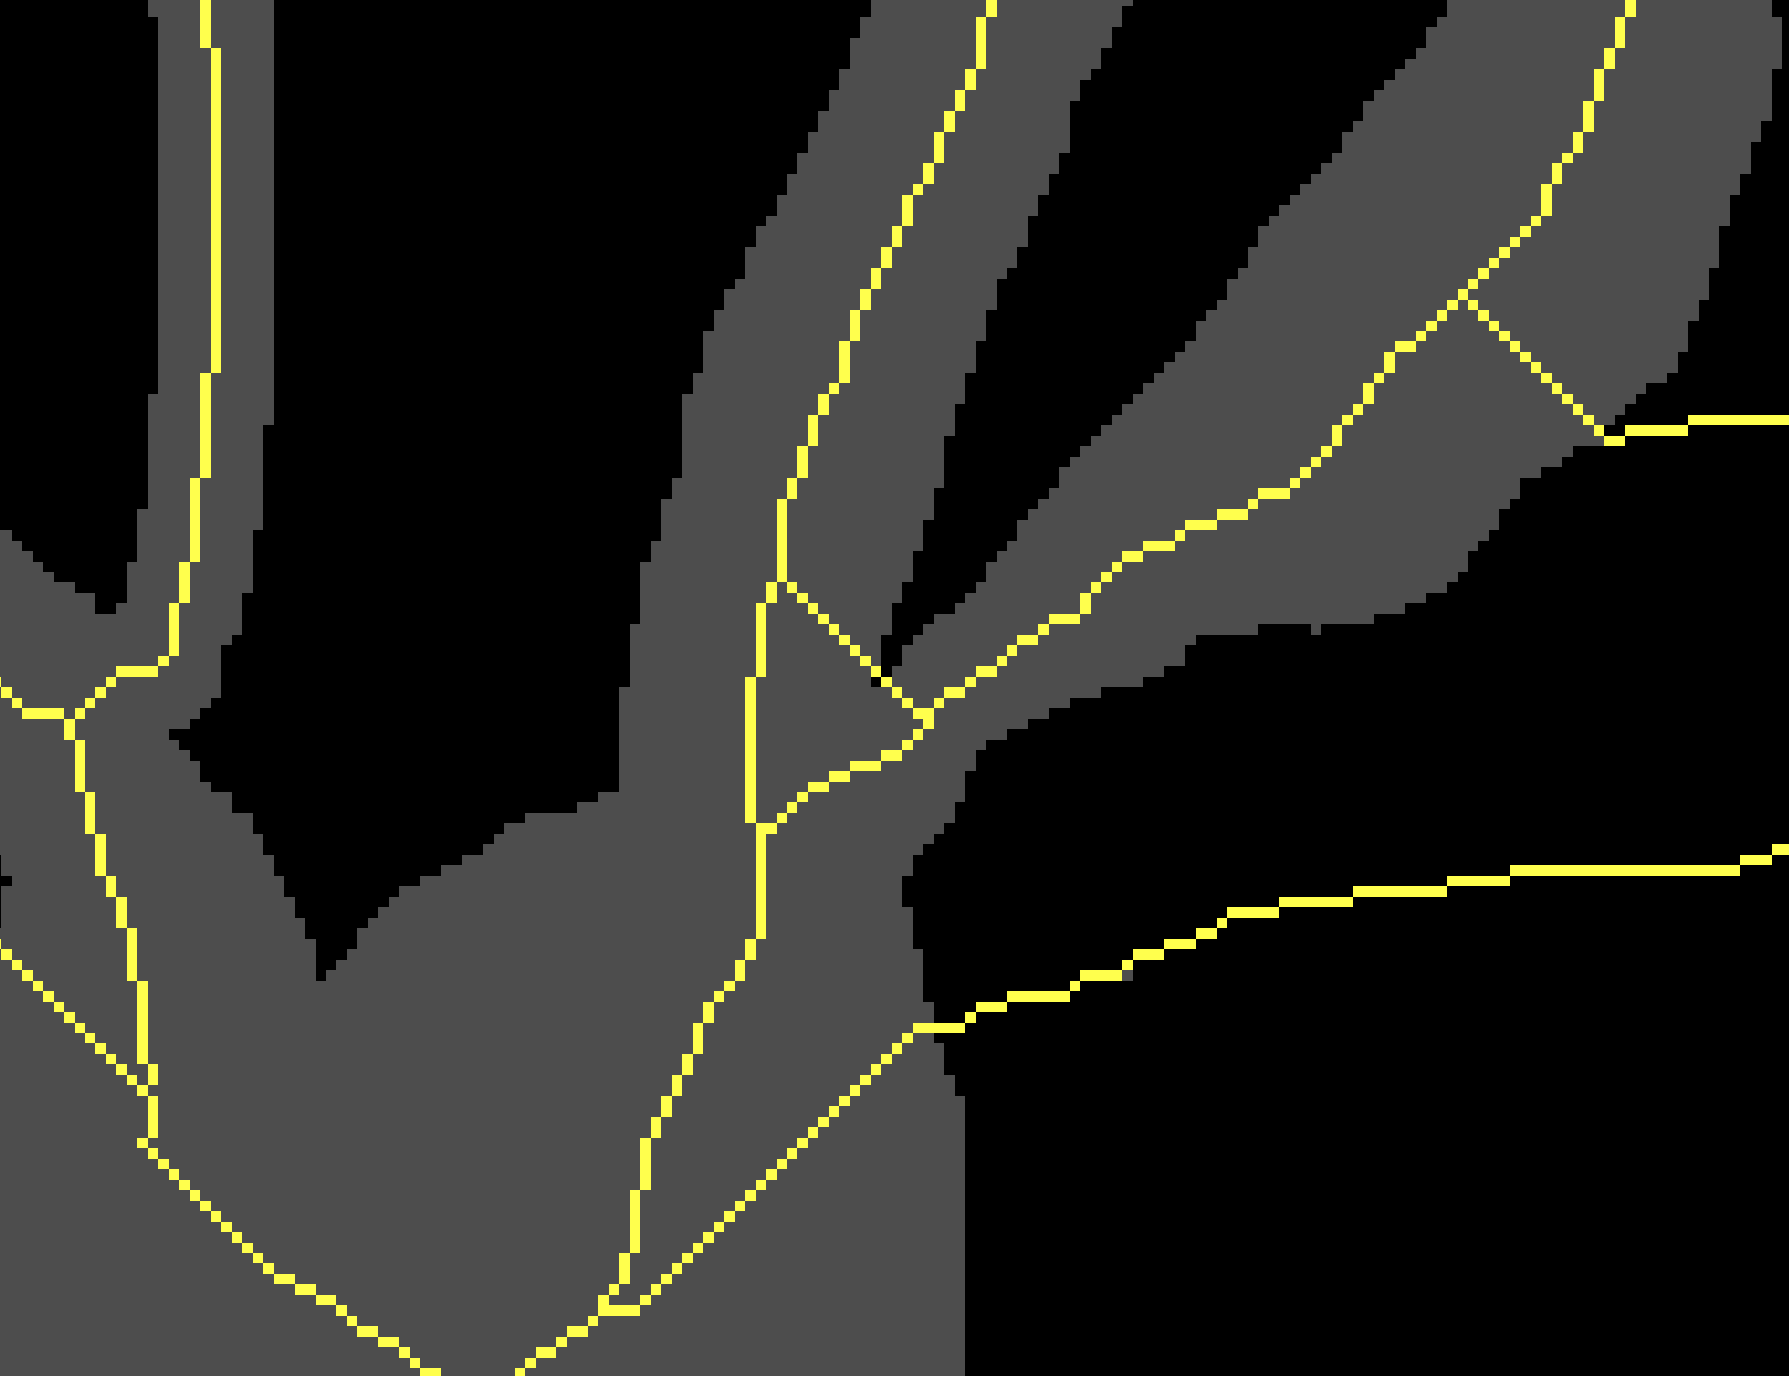
\includegraphics[width=\linewidth]{figures/no_junction_cleanup.png}
    \caption{Before cleanup}
    \label{fig:junction_cleanup:a}
  \end{subfigure}
  \hfill
  \begin{subfigure}[b]{0.4\linewidth}
    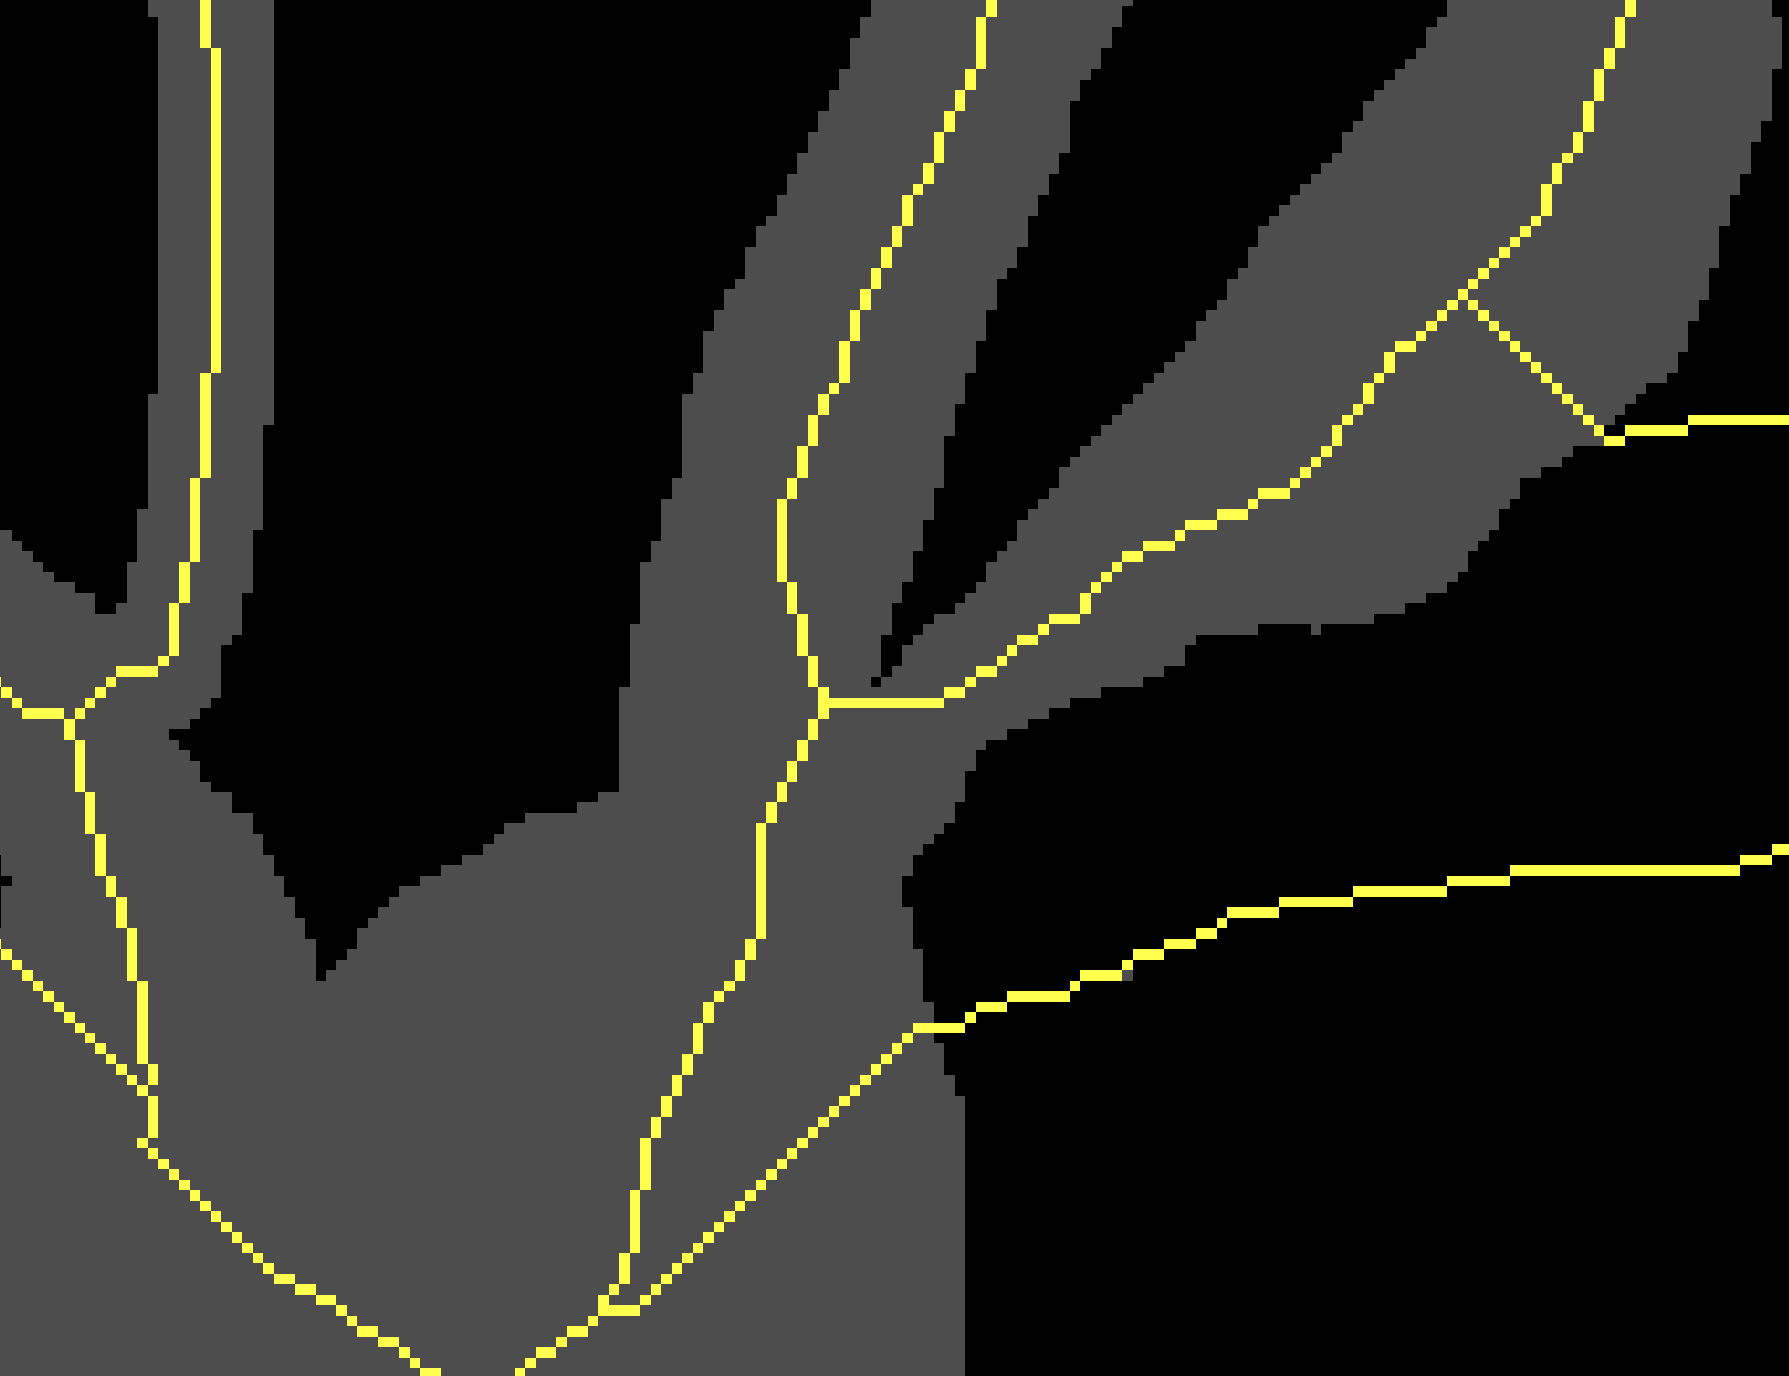
\includegraphics[width=\linewidth]{figures/junction_cleanup.png}
    \caption{After cleanup}
    \label{fig:junction_cleanup:b}
  \end{subfigure}
  \caption[Junction cleanup removes triangle artifacts]{Junction
    cleanup removes triangle artifacts. (a) A triangle artifact at
    a vessel bifurcation after thinning. (b) After cleanup, the artifact
    is removed and the skeleton correctly represents the bifurcation
  topology.}
  \label{fig:junction_cleanup}
\end{figure}

A key observation from our experiments is that hole filling alone
resolves the vast majority of skeletonization artifacts before they
appear in the graph. When preprocessing is active, junction cleanup
becomes redundant for most images. This makes mask-level
preprocessing the primary and most effective defense against thinning
artifacts, with junction cleanup serving as a secondary safety net
for the remaining edge cases.

\subsection{Skeletonization Performance}\label{sec:results:performance}

We evaluated VesSkel's thinning performance on 2D and 3D data against
three competing implementations: scikit-image's~\cite{skimage}
Lee~\cite{lee94} and Zhang~\cite{zhang84} methods, and VesselVio's
Lee94 implementation~\cite{VesselVio}.

For 2D evaluation we used the full HRF dataset (45 images, $3504
\times 2336$~px each). Table~\ref{tab:perf-2d} reports the mean
thinning time per image. VesSkel achieves a mean of 0.084~s,
outperforming the next-fastest implementation (scikit-image Zhang,
0.157~s) by 1.87$\times$. Compared to the widely used Lee94 baseline
in scikit-image (0.438~s), VesSkel is 5.21$\times$ faster; against
VesselVio's Lee94 (0.796~s) the speedup reaches 9.46$\times$.

\begin{table}[htb]
  \centering
  \caption{2D thinning benchmark on the HRF dataset (45 images).}
  \label{tab:perf-2d}
  \small
  \begin{tabularx}{0.7\linewidth}{lcc}
    \toprule
    Implementation & Mean time (s) & vs.\ VesSkel \\
    \midrule
    VesSkel (Lee94)     & 0.084 & ---   \\
    skimage Zhang       & 0.157 & 1.87$\times$ slower \\
    skimage Lee         & 0.438 & 5.21$\times$ slower \\
    VesselVio Lee94     & 0.796 & 9.46$\times$ slower \\
    \bottomrule
  \end{tabularx}
\end{table}

For 3D evaluation we used a binarized vessel segmentation volume from
VesSAP~\cite{VesSAP} ($600\times304\times325$~voxels). Mean times
over 10 runs are shown in Table~\ref{tab:perf-3d}.~VesSkel (0.730~s)
is competitive with scikit-image (1.024~s) and VesselVio (0.804~s).

\begin{table}[htb]
  \centering
  \caption{3D thinning benchmark on the VesSAP test volume
  ($600\times304\times325$).}
  \label{tab:perf-3d}
  \small
  \begin{tabularx}{0.7\linewidth}{lcc}
    \toprule
    Implementation & Mean time (s) & vs.\ VesSkel \\
    \midrule
    VesSkel (Lee94)   & 0.730 & ---   \\
    skimage Lee       & 1.024 & 1.40$\times$ slower \\
    VesselVio Lee94   & 0.804 & 1.10$\times$ slower \\
    \bottomrule
  \end{tabularx}
\end{table}

Critically, VesSkel sacrifices no correctness for speed. The output
is~\textbf{bit-identical} to scikit-image's Lee94 implementation.
This was verified via the regression test suite described in
Section~\ref{sec:methods:impl:tests}.

Beyond per-image thinning, the \texttt{vesskel run} CLI supports
parallel batch processing. On our test machine, processing all 45
HRF images took 166.7~s with a single worker and 103.7~s with 12
workers (1.61$\times$ speedup).

This sub-linear speedup probably stems from the heterogeneous CPU
architecture of our test-machine (only 2 Performance-cores and 8
Efficiency-cores) and the fact that Numba already parallelizes the
thinning of each individual image, so multi-worker gains are
partially offset by inter-process contention. On homogeneous
multi-core workstations, the speedup may approach the worker count more closely.

\subsection{Skeleton and Graph Features}\label{sec:results:features}

- Tabelle in appendix und nur "summary" der tools erwähnen -> anzahl
gesamtfeatures aller tools und nur in vesskel eingebaute features als
"relevant" erwähnen und grobe unterteilung hier erwähnen:
- topology: nodes, edges, endpoints, bifurcations
- morphology: lengths, tortuosity, radii, fractal dimension, HGU
- density: vessel area fraction

\subsection{Phenotype Differentiation}\label{sec:results:phenodiff}

- ANOVA: which features discriminate best between groups
- figure: feature distribution differences for phenotypes (nur die top anova!)
- correlation heatmap, summary tables -> könnte zu lang werden, aufs
wichtigste beschränken!
- key findings zusammenfassen
- nur zeugs was raussticht erwähnen, tabellen etc. in appendix und referenzieren

\subsection{Pheontype Classification}\label{sec:results:phenoclass}

- Multi-class cross-validated classifier comparison: RF, SVM,
Logistic Regression, ensembling
- Table: per-classifier accuracy (5-fold CV). Best model achieves X% accuracy.
- (ROC curves, confusion matrices, feature importance)
- Best-performing model and key predictive features

\section{Discussion}\label{sec:discussion}

% The discussion typically starts with a summary of your work's most
% important results. Then, you discuss limitations of your work and
% potential follow-up. Finally, you end on a positive note and tell the
% reader at a very high abstraction level how your work advanced the
% field: What did we learn through your work? What do we know now that
% was not known before? Which type of analyses can now be run now that
% were not possible before?
%
% Typically, discussions are internally unstructured. But you may
% deviate from this rule of thumb, e.\,g., by including separate
% subsections on limitations and outlook.

- Summary of main findings: VesSkel enables fully reproducible,
quantitative vessel phenotype analysis
- Feature set captures biologically relevant differences between clinical groups
- Limitations: small dataset (45 images), 2D-only validation on
fundus, no longitudinal data
- Potential follow-ups: wavefront -> 3d performance

\section{Methods}\label{sec:methods}

% \subsection{Structure of the Methods section}
%
% Good Methods sections are designed in such a way that the subsection
% headings allow the reader to quickly navigate it without reading the
% entire section from top to bottom. You may think of it as a
% dictionary where readers look up details of the work that are of
% particular interest to them. Each individual subsection should be
% detailed enough to allow replication of your work, so be precise in
% your descriptions. Overall, the subsections of your Methods section
% should cover all methodological details that are relevant for your
% work: details on your ML model or algorithm, descriptions of datasets
% and data preprocessing, details on evaluation protocols and metrics,
% description of competitor approaches, etc.
%
% \subsection{Equations}
%
% When using mathematical formalism, make sure that you always define
% all symbols, including indices. For instance, if for some reason you
% want to introduce the quantity $s$ as the sum of all Fibonacci
% numbers $F_i$ with odd indices smaller or equal to $100$, you should
% not simply write
% \begin{equation}
%   s=\sum_{i}F_i \label{eq:bad}
% \end{equation}
% and hope that the range of the index $i$ is clear from the context.
% Instead, introduce an index set
% $\mathcal{O}_{100}=\{i\in\mathbb{N}\mid i\leq100\land\text{$i$ is
% odd}\}$ and define $s$ as in the following \Cref{eq:good}:
% \begin{equation}
%   s=\sum_{i\in\mathcal{O}_{100}}F_i \label{eq:good}
% \end{equation}
%
% Moreover, it is preferable to always use numbered instead of
% unnumbered equation environments (i.\,e.,
%   \verb|\begin{equation}...\end{equation}| and
%   \verb|\begin{align}...\end{align}| instead of
%   \verb|\begin{equation*}...\end{equation*}| and
% \verb|\begin{align*}...\end{align*}|). Like this, you can reference
% the equations in the text and it is easier for readers to refer to them.
%
% \subsection{Theorems, definitions, proofs, and similar environments}
%
% This template provides \verb|definition|, \verb|observation|,
% \verb|remark|, \verb|proposition|, \verb|lemma|, \verb|theorem|, and
% \verb|proof| environments you can use as needed. Examples are
% provided in \Cref{def:dummy-def} and \Cref{thm:dummy-theorem}.
%
% \begin{definition}[Optional name of defined concept]\label{def:dummy-def}
%   Statement of the definition.
% \end{definition}
%
% \begin{theorem}[Optional name of theorem]\label{thm:dummy-theorem}
%   Statement of the theorem.
% \end{theorem}
%
% \begin{proof}
%   Proof here.
% \end{proof}

\subsection{Lee94 Thinning Algorithm}\label{sec:methods:lee}

The Lee94 algorithm~\cite{lee94} produces topologically
preserving skeletons by iteratively removing border pixels from a
binary shape until only a one-voxel-wide medial axis remains. The
algorithm proceeds in six directional sub-iterations (north, south,
east, west, up, down). In each sub-iteration, a border pixel is
removed only if it satisfies four criteria:
(1)~it is a \textbf{border point} (at least one 4-/6-neighbor is
background), (2)~it is \textbf{not an endpoint} (more than one
foreground neighbor in the 8-/26-neighborhood),
(3)~removing it leaves the \textbf{Euler characteristic} unchanged
($\Delta\chi = 0$, preventing hole or tunnel creation), and
(4)~it is a \textbf{simple point} (the foreground neighbors form a
single connected component, preventing disconnection). In 3D,
conditions~(3) and~(4) are complementary; in 2D,
condition~(3) is redundant (see below).

\subsection{Implementation Details}\label{sec:methods:impl}

\paragraph{Deviations of this Implementation}\label{sec:methods:impl:deviations}

Our 2D implementation differs from the canonical Lee94 algorithm in
two important ways. First, we proved that the Euler invariant check
is redundant in 2D (full proof in the project documentation). In 2D,
a hole cannot be created by removing a border point (any border point
has at least one background 4-neighbor, providing an escape path), and
a hole cannot be eliminated by removing a simple point (the
simple-point condition already prevents disconnection). Since
$\Delta\chi = \Delta O - \Delta H$ and $\Delta H = 0$ always holds,
the simple-point condition ($\Delta O = 0$) guarantees $\Delta\chi =
0$. Omitting the Euler check removes the need for octree construction
and Euler LUT lookups, contributing directly to the 2D speedups
reported in Section~\ref{sec:results:performance}.

Second, 2D images are processed natively as 2D arrays rather than
embedded in a 3D volume. This collapses the 26-neighborhood to an
8-neighborhood, reduces border detection from six directions to four,
and halves memory usage.

% TODO: add 3D details

\paragraph{Numba-Parallelized Implementation}\label{sec:methods:impl:numba}

- actual implementation details
- simple point ist 26-adjacency connectivity in 3D; 8-adjacency in 2D via LUT

\paragraph{Tests}\label{sec:methods:impl:tests}

- Correctness verified against scikit-image Lee94 output -> tests erwähnen

\subsection{Cleanup Steps}\label{sec:methods:cleanup}

Binary vessel masks frequently contain small holes and gaps
introduced during segmentation that would produce circular skeleton
artifacts during thinning (Section~\ref{sec:results:cleanup}).
VesSkel addresses these through optional preprocessing operations
applied before skeletonization. Hole filling
(\texttt{scipy.ndimage.binary\_fill\_holes}) fills all enclosed
background regions in the mask. To preserve legitimate anatomical
voids, the \texttt{max\_hole\_size} parameter reverts filled holes
whose area exceeds a configurable threshold. VesSkel also offers
morphological closing (\texttt{scipy.ndimage.binary\_closing}) as an
additional preprocessing step; however, on the HRF dataset
experiments showed no noticeable improvement over hole filling alone,
so closing was disabled (\texttt{closing\_iterations = 0}) in our
experiments. We used \texttt{max\_hole\_size = 300}.

Some thinning-induced artifacts, particularly small triangle
structures at bifurcation points, may survive mask-level
preprocessing. VesSkel removes these by analyzing the skeleton graph
after thinning. The skeleton is converted to a NetworkX graph $G =
(V, E)$ via Skan's \texttt{skeleton\_to\_nx} function~\cite{Skan<3},
and all elementary cycles $\mathcal{C}$ are enumerated using
\texttt{networkx.\\cycle\_basis}. For a cycle $c = (v_1, \dots, v_n)
\in \mathcal{C}$ with $v_{n+1} = v_1$, the perimeter is
\[
  P(c) = \sum_{i=1}^{n} \lVert \operatorname{pos}(v_{i+1}) -
  \operatorname{pos}(v_i) \rVert_2
\]
and the local vessel diameter is estimated as
\[
  D(c) = \frac{2}{n} \sum_{i=1}^{n}
  \operatorname{EDT}(\operatorname{pos}(v_i)),
\]
where $\operatorname{pos}(v)$ gives the pixel coordinates of node $v$
and $\operatorname{EDT}$ is the Euclidean distance transform of the
vessel mask. A cycle is classified as an artifact if
\[
  P(c) < \tau \cdot D(c)
\]
with a default threshold of $\tau = 2.5$. Each such cycle --- or
connected group of overlapping cycles --- is collapsed to a single
pixel at its geometric centroid. External edges previously connected
to the removed nodes are reconnected to this centroid via Bresenham
line rasterization, preserving graph connectivity.

\subsection{Graph Construction and Features}\label{sec:methods:graph}

- Build vessel graph via skan (Skeleton object -> CSR graph).
- Features computed: node degree, edge length (branch-distance),
tortuosity (branch/euclidean ratio), vessel radii (distance
transform), fractal dimension (box-counting, log-log slope), HGU
(total length / endpoint count).
- selbst implementiertes zeugs genauer erläutern

\subsection{Dataset and Preprocessing}\label{sec:methods:data}

We evaluate VesSkel on two datasets. The primary evaluation uses the
High-Resolution Fundus (HRF) dataset~\cite{HRF}, which comprises 45
fundus images ($3504 \times 2336$~px) with corresponding manual
vessel segmentation masks and field-of-view masks. The dataset
includes three clinical groups of 15 images each: healthy subjects,
patients with diabetic retinopathy, and patients with glaucoma. These
conditions are known to alter retinal vessel morphology, providing a
suitable test bed for phenotype analysis.

For 3D benchmarking, we use a test volume from the VesSAP
Repository~\cite{VesSAP} ($600\times304\times325$~voxels), which we
binarized, and the scikit-image brain volume~\cite{skimage}.

Preprocessing follows the procedure described in
Section~\ref{sec:results:cleanup}. Binary vessel masks are first
masked by the provided field-of-view mask to exclude regions outside
the retina. Hole filling removes enclosed background regions while
preserving anatomical voids. Closing is disabled since the HRF manual
segmentations contain few gaps.

\subsection{Experimental Setup}\label{sec:methods:setup}

\paragraph{Runtime Tests}\label{sec:methods:setup:runtime}

All benchmarks were run on a notebook equipped with an Intel Core
i5-1235U (12 cores: 2 P-cores, 8 E-cores; 16~GB RAM) running Arch
Linux (kernel 7.0.12).~Times were measured with
\texttt{time.perf\_counter} with Numba's JIT compiler warmed up on a
synthetic $10\times10$ (2D) or $10\times10\times10$ (3D) binary cube
before timing.

For parallel batch processing, the \texttt{vesskel run} CLI exposes a
\texttt{-{}-jobs} (\texttt{-j}) flag that defaults to the number of
available CPU cores.~Each worker processes one image independently
using a shared Numba JIT cache, so inter-process I/O is the primary
overhead.~The sub-linear speedup on our test machine (1.61$\times$ with
12 workers) reflects the hybrid CPU architecture (2 P-cores, 8
E-cores); on homogeneous multi-core workstations the speedup approaches
the worker count more closely.

\paragraph{Phenotype Differentiation}\label{sec:methods:setup:phenodiff}

- anova

\paragraph{Phenotype Prediction}\label{sec:methods:setup:phenoclass}

- classifiers: Random Forest/SVM/LogReg/Stacking classifiers with
5-fold stratified cross-validation -> erwähnen, dass aus sklearn genommen

\section{Code availability}\label{sec:code}

% If you wrote any source code as part of your work, provide a link to
% a well-documented GitHub repository here. Moreover, release a stable
% version of your source code and provide its DOI here. You can use
% Zenodo for this, see \url{https://help.zenodo.org/docs/github/}.
% Write ``Not applicable'' if and only if you did not write any source
% code as part of your work.

- GitHub repository und PyPi link, Zenodo DOI.
- Installation via `uv` oder `pip`, napari plugin, CLI batch processing.

\section{Data availability}\label{sec:data}

% Describe from where you obtained the public data underlying your
% work. Your descriptions should be detailed enough to allow others to
% access the exact same data and to reproduce your results, using the
% code you linked in \Cref{sec:code}. If you generated data yourself
% (e.g., through simulation), either deposit the data in a public
% repository such as Zenodo and provide the DOI here or explain how
% others can rerun the simulation to generate the data themselves. If
% you used private or sensitive data that is not public and cannot be
% made publicly available, explain why this is the case. Write ``Not
% applicable'' if and only if you did not use any data for your work.

- HRF dataset reference (Budai et al., 2013), CC-BY 4.0.

\printbibliography

\clearpage

\appendix
\renewcommand{\thefigure}{S\arabic{figure}}
\renewcommand{\thetable}{S\arabic{table}}
\setcounter{figure}{0}
\setcounter{table}{0}
\crefalias{section}{appendix}
\crefname{appendix}{appendix}{appendices}
\Crefname{appendix}{Appendix}{Appendices}

\section{Supplementary figures}\label{appendix:figures}

% Supplementary figures that provide additional results but do not fit
% into the narrative of the main text can be put here. All
% supplementary figures should be referenced from the main text and
% should be listed here in the order of these references. Delete this
% section if not needed.
%
% \begin{figure}[htb]
%   \centering
%   \includegraphics[width=0.5\linewidth]{example-image-b}
%   \caption{Caption of \Cref{fig:supp-fig}.}
%   \label{fig:supp-fig}
% \end{figure}

\section{Supplementary tables}\label{appendic:tables}

% Supplementary tables that provide additional results but do not fit
% into the narrative of the main text can be put here. All
% supplementary tables should be referenced from the main text and
% should be listed here in the order of these references. Delete this
% section if not needed.
%
% \begin{table}[htb]
%   \centering
%   \caption{Example of a table generated with the \texttt{tabular}
%     environment that has a slightly simpler syntax than the
%     \texttt{tabularx} environment but does not support flexible-width
%   columns.}\label{tab:supptab}
%   \begin{tabular}{lll}
%     \toprule
%     Column 1 & Column 2 & Column 3\\
%     \midrule
%     X & Y & Z \\
%     \bottomrule
%   \end{tabular}
% \end{table}

\clearpage

\section{AI usage declaration}\label{sec:ai-declaration}

Gemini, Chatgpt, GitHub Copilot, Deepseek, Opencode

In the boxes below, please specify which AI tool you used, to what
extent, and for which task. If you did not use AI tools for the task,
please state so by writing \textit{``I did not use any AI tools for
this task''} in the corresponding box. Examples of AI tools to
declare: ChatGPT, Claude, Gemini, Microsoft Copilot, Grammarly,
DeepL, Google Translate, Perplexity, Elicit, Explainpaper, and
ResearchRabbit. Example sentences:

\begin{itemize}
  \item Task: Review and editing of the text: \textit{``I used
      Grammarly for proofreading, revising the grammar of the text in
      \Cref{sec:introduction,sec:discussion}, and for rewording
    convoluted sentences throughout this work.''}
  \item Task: Structuring and planning the text: \textit{``I used
      Claude to suggest how my background description in
    \Cref{sec:introduction} should be structured and what should be included.''}
  \item Task: Coding: \textit{``I used the Microsoft Copilot
      extension in my IDE for code completion and for generating the
    code for the JavaScript frontend.''}
\end{itemize}

\vspace{.25em}

\begin{answerbox}{Task: Brainstorming and concept development}
  Tools used for the development of ideas, obtaining research goals,
  objectives, designing the research, and identifying and defining
  relevant concepts.
\end{answerbox}

\vspace{.25em}

\begin{answerbox}{Task: Literature review and analysis}
  Tools used for identifying relevant literature, reviewing
  potentially relevant literature,  and creating summaries.
\end{answerbox}

\vspace{.25em}

\begin{answerbox}{Task: Methodology}
  Tools used for identifying a suitable methodology and developing
  and adapting the methodology to the research question(s).
\end{answerbox}

\vspace{.25em}

\begin{answerbox}{Task: Coding}
  Tools used for writing and documenting code, algorithms, and
  software, testing and debugging, and understanding existing code.
\end{answerbox}

\vspace{.25em}

\begin{answerbox}{Task: Data collection, generation, and analysis}
  Tools used for collecting, generating, and processing primary or
  secondary data. Tools for qualitative or quantitative data analysis.
\end{answerbox}

\vspace{.25em}

\begin{answerbox}{Task: Interpretation and validation}
  Tools used for interpreting results, deriving implications, and
  assessing general replicability and reproducibility of the results
  or other research findings.
\end{answerbox}

\vspace{.25em}

\begin{answerbox}{Task: Structuring and planning the text}
  Tools used for generating the outline of the work and/or the
  outline of specific sections.
\end{answerbox}

\vspace{.25em}

\begin{answerbox}{Task: Text generation}
  Tools used for generating text on various topics in different
  sections of the work, including titles and abstracts.
\end{answerbox}

\vspace{.25em}

\begin{answerbox}{Task: Translating text}
  Tools used for translating text written by the author or by others.
\end{answerbox}

\vspace{.25em}

\begin{answerbox}{Task: Review and editing of the text}
  Tools used for critically reviewing the written text, obtaining
  feedback, revising the content, structure, or grammar of the text,
  proofreading, rewording or paraphrasing the given text, and
  shortening or expanding the text.
\end{answerbox}

\vspace{.25em}

\begin{answerbox}{Task: Bibliography management}
  Tools used to create or format the reference list.
\end{answerbox}

\vspace{.25em}

\begin{answerbox}{Task: Other activities}
  Tools used for anything not covered by the given tasks.
\end{answerbox}

\clearpage

\section{Declaration of academic integrity}\label{sec:declaration}

I hereby declare that I have authored this work independently and
without the use of any sources or assistance other than those
specifically cited. All content taken verbatim or paraphrased from
other sources has been clearly identified as such. Furthermore, I
certify that this work has not been submitted, in its current or a
similar form, for any other examination. All usage of AI tools has
been fully disclosed in \Cref{sec:ai-declaration}, and I take full
responsibility for all content generated with the help of AI. I am
aware that any false or incomplete declarations given here or in
\Cref{sec:ai-declaration} may be treated as attempts at deception and
could thus lead to the failure of this examination. I am also aware
that inability to provide in-depth technical explanations for any
content contained in this work or in the underlying source code may
be treated as evidence for illicit AI usage or misappropriation of
the work of others and could thus lead to the failure of this examination.

\namesigdate{[Your name]}

\end{document}
